\documentclass[xcolor={dvipsnames}]{beamer}
    \usepackage{tikz}
    \usepackage{multimedia}
    \usepackage{hyperref}
    \usepackage{array}
    \usepackage[MeX]{polski}
    \usepackage[utf8]{inputenc}
    \usepackage{graphicx}
    \usepackage[T1]{fontenc}
    \usepackage{color}
    \usepackage{amsthm}
    \usetheme{CambridgeUS}
    \setbeamercolor*{structure}{bg=PineGreen!20,fg=PineGreen}
    \usepackage{color}
    \usepackage{outlines}
    \usepackage{mathtools}
    
    \setbeamercolor*{palette primary}{use=structure,fg=white,bg=structure.fg}
    \setbeamercolor*{palette secondary}{use=structure,fg=white,bg=structure.fg!75}
    \setbeamercolor*{palette tertiary}{use=structure,fg=white,bg=structure.fg!50!black}
    \setbeamercolor*{palette quaternary}{fg=white,bg=black}
    
    \setbeamercolor{section in toc}{fg=black,bg=white}
    \setbeamercolor{alerted text}{use=structure,fg=structure.fg!50!black!80!black}
    \setbeamercolor{block title alerted}{use=structure, fg=structure.fg ,bg=red}
    
    \setbeamercolor{titlelike}{parent=palette primary,fg=structure.fg!50!black}
    \setbeamercolor{frametitle}{bg=gray!10!white,fg=PineGreen}
    
    \setbeamercolor*{titlelike}{parent=palette primary}
    \setbeamertemplate{enumerate items}[default]

    
    
\author{Arkadiusz Popczak}
\title{Stała Fermiego}
\date{22.11.2018}
\begin{document}
\begin{frame}
    \maketitle
\end{frame}

\begin{frame}{Agenda}

    \begin{outline}[enumerate]

        \1 Teoria Fermiego
            \2 Rozpad $\beta^-$
            \2 Doświadczenie Wu
        \1 Stała Fermiego
            \2 Definicja
            \2 Niepewności
        \1 Eksperymenty
            \2 Lata 80
            \2 Eksperymrnt FAST
            \2 Eksperyment MuLan


    \end{outline}

\end{frame}

\begin{frame}{Teoria Fermiego}{Rozpad $\beta^-$}

    W roku 1933 Enrico Fermi \cite{fermi} zaproponował opis rozpadu $\beta^-$. Na poziomie atomowym:

    \begin{figure}

        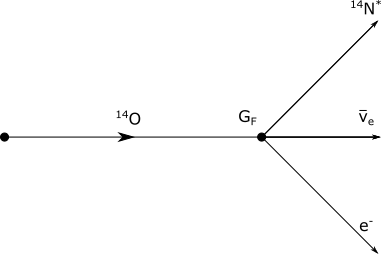
\includegraphics[scale=0.8]{4points.png}

    \end{figure}

\end{frame}

\begin{frame}{Teoria Fermiego}{Rozpad $\beta^-$}

    Na poziomie nukleonów:

    \begin{figure}

        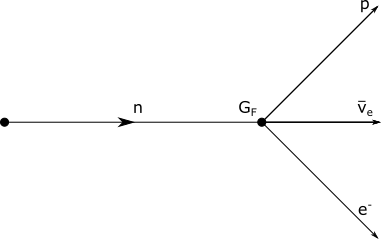
\includegraphics[scale=0.9]{4pointsnuc.png}

    \end{figure}

\end{frame}

\begin{frame}{Teoria Fermiego}{Rozpad $\beta^-$}

Uniwersalne sprzężenie punktowe pozostawiło nam jeden wolny parametr $G_F$. Teoria Fermiego zakładała, że oddziaływania słabe mają tą samą symetrię co oddziaływania elektormagnetycznie. Zmieniło się to w roku 1957.

\end{frame}

\begin{frame}{Teoria Fermiego}{Doświadczenie Wu}

Pani C.S.Wu zaobserwowała łamanie parzystości w rozpadzie:\\
\centering
\begin{math}
\prescript{60}{}Co \rightarrow \prescript{60}{}Ni + e^- + \bar{v}_e
\end{math} \cite{wuexp}

\begin{figure}
    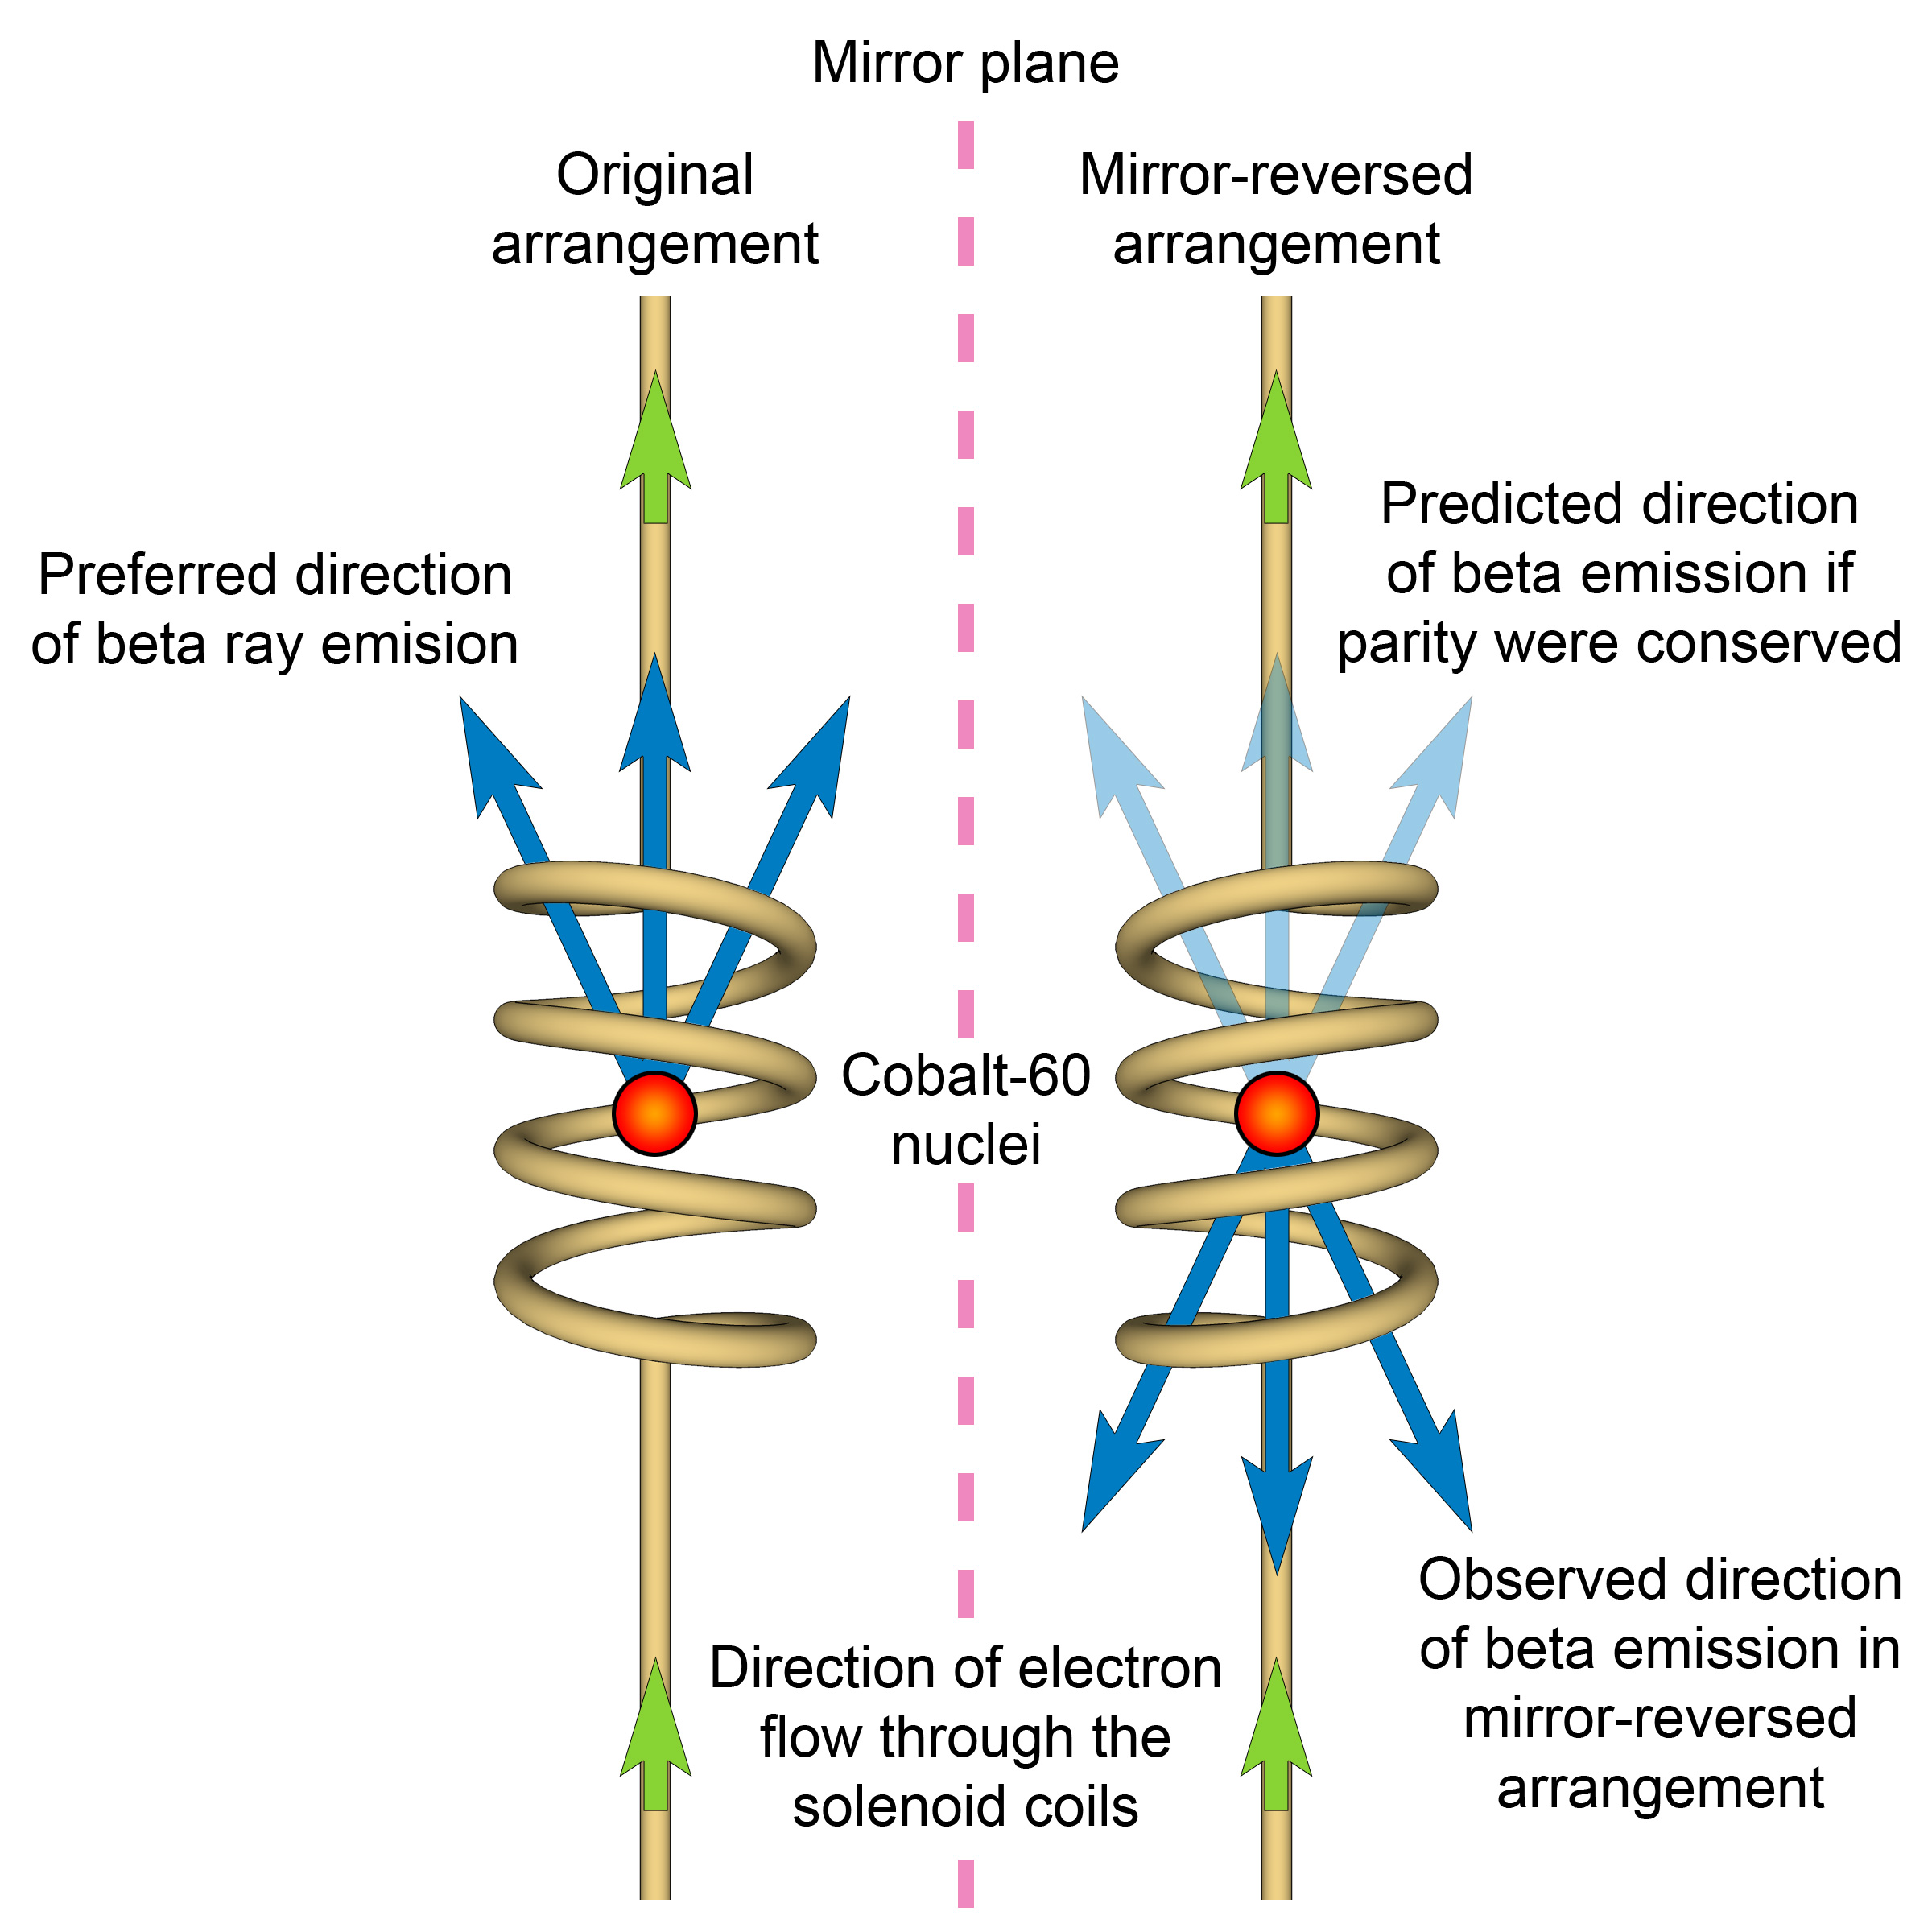
\includegraphics[scale=0.06]{Wu_experiment.jpg}
\end{figure}

\end{frame}

\begin{frame}{Stała Fermiego}{Definicja}

        Stała Fermiego $G_F$ jest zdefiniowana poprzez równanie:\\


\centering
\begin{math}
        \tau_\mu^{-1} \equiv \frac{G_F^2 m_\mu^5}{192 \pi^3}(1 + \Delta q),
\end{math}\\


\raggedright
    Gdzie $\Delta q$ jest obliczana z lagranżjanu teorii Fermiego i zawiera poprawki QCD i QED. \cite{strauts}
\end{frame}


\begin{frame}{Eksperymenty}{Lata 80}
    W latach 90 przeprowadzono dwa eksperymenty:

    \begin{outline}[enumerate]
        \1 Oba przeprowadzono w 1984 roku.
        \1 Przez 20 lat nie otrzymano lepszego wyniku.
        \1 Ograniczenia teoretyczne.

    \end{outline}

    Pozwoliło to oszacować stałą Fermiego na poziomie $\frac{\Delta G_F}{G_F}$ = 18 ppm.

\end{frame}

\begin{frame}{Eksperymenty}{Lata 80}

    \begin{figure}
        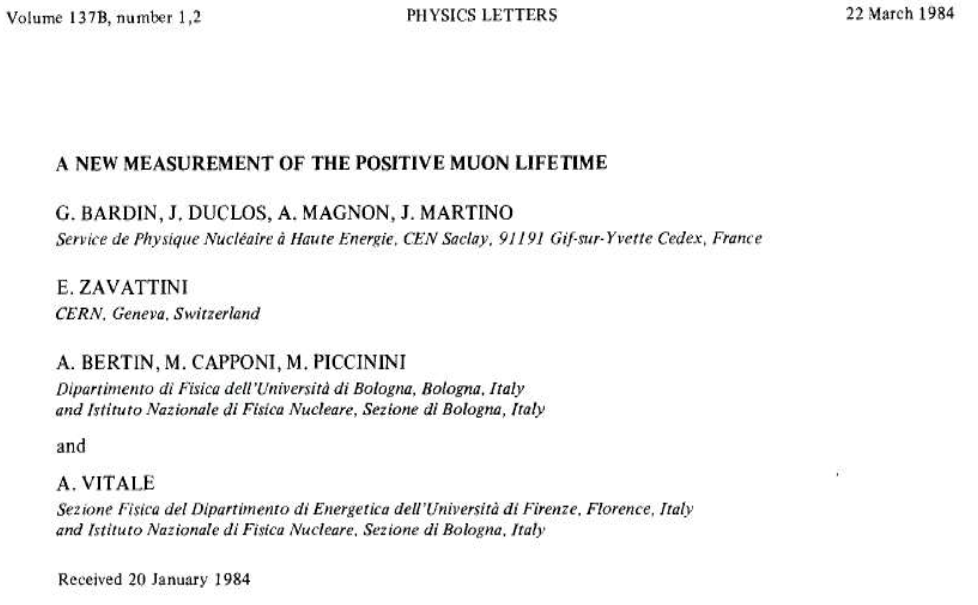
\includegraphics[scale=0.7]{positive1_bardin.PNG}

    \end{figure}

\end{frame}

\begin{frame}{Eksperymenty}{Lata 80}

    Wykorzystano strumień pionów, które po rozpadzie na mion zatrzymywały się na tarczy a następnie do rozpaday się na pozyton. Najważniejsze informacje:
    
    \begin{outline}[enumerate]
        
        
    \end{outline}

\end{frame}

\begin{frame}{Eksperymenty}{Eksperymrnt FAST}

\end{frame}

\begin{frame}{Eksperymenty}{Eksperyment MuLan}

\end{frame}


\begin{frame}{Bibliografia}

    \begin{thebibliography}{9}
        \setbeamertemplate{bibliography item}[text]

        \bibitem{fermi} Yang, C. N  "Fermi's $\beta$-decay Theory". Asia Pacific Physics Newsletter. 1 (01): 27–30

        \bibitem{wuexp}  Wu, C. S.; Ambler, E; Hayward, R. W.; Hoppes, D. D.; Hudson, R. P. (1957). "Experimental Test of Parity Conservation in Beta Decay". Physical Review. 105 (4): 1413–1415.

        \bibitem{strauts} T. van Ritbergen and R. G. Stuart, Nucl. Phys.B564,343 (2000); T. van Ritbergen and R. G. Stuart, Phys.Lett.B437,  201  (1998);   T. van  Ritbergen  andR. G. Stuart, Phys. Rev. Lett.82, 488 (1999).

    \end{thebibliography}

\end{frame}

\end{document}
